% !TeX root = ../../../main.tex

The foundational deep-inelastic scattering experiments at the SLAC linear collider
in the late 60s and early 70s demonstrated the presence inside the
proton of pointlike  constituents, soon identified with quarks, the
elementary particles that interact and are bound inside the proton by
gluons, the carriers of the strong  nuclear force.
%
It was rapidly clear, and confirmed in detail by subsequent studies,
that these pointlike constituents, collectively called ``partons'' by
Feynman~\cite{Feynman:1969wa}, include the up and down quarks that
carry the proton quantum numbers, but also gluons, as well
as an infinite number of pairs of quarks and their
antimatter counterparts, antiquarks.
%
The description of electron-proton and proton-proton collisions at high
momentum transfers in terms of collisions between partons is now rooted in the
theory of Quantum  Chromodynamics (QCD), and it provides the basis of
modern-day precision phenomenology at proton accelerators such as the
\acrfull{lhc} of \cern~\cite{Gao:2017yyd} as well as for future facilities
including the \eic~\cite{AbdulKhalek:2021gbh}, the FPF~\cite{Feng:2022inv}, and 
neutrino telescopes~\cite{IceCube-Gen2:2020qha}.

Knowledge of the structure of the proton, which is necessary in order
to obtain
quantitative prediction for physics processes at the \lhc and other
experiments, is encoded in
the distribution of  momentum carried by partons of each type
(gluons, up quarks, down quarks, up antiquarks, etc):
parton distribution functions (\pdfs).
%
These \pdfs could be in principle
computed from first principles, but in
practice even their determination from numerical
simulations~\cite{Constantinou:2020hdm} is extremely challenging.
%
Consequently,  the only 
strategy currently available for obtaining the
reliable determination of the proton \pdfs which is required to evaluate \lhc
predictions is empirical, through the global analysis of
data for which precise theoretical predictions and experimental
measurements are available, so that the \pdfs are the only
unknown~\cite{Gao:2017yyd}.

While this successful framework has by now been worked through in great detail, several key open questions remain open.
%
One of the most controversial of these concerns the treatment of
so-called heavy quarks, i.e.\ those whose mass is greater than that of
the proton ($m_p=0.94$~GeV). Indeed, virtual quantum effects and
energy-mass considerations suggest that the three light quarks and
antiquarks (up, 
down, and strange) should all be present in the proton
wave-function.
%
Their \pdfs are therefore surely determined by the low-energy
dynamics that controls the nature of the proton as a bound
state.
%
However, it is a well-known fact~\cite{DeRoeck:2011na,
  Kovarik:2019xvh,Gao:2017yyd,Rojo:2019uip}
that in high enough energy collisions all species of quarks can be
excited and hence observed
inside the proton, so their \pdfs are nonzero.
%
This excitation
follows from standard QCD radiation and it can be computed accurately
in perturbation theory.

But then the question arises: do heavy quarks also contribute to the
proton wave-function? Such a contribution is called ``intrinsic'', to
distinguish it from that computable in
perturbation theory, which originates from QCD radiation.
%
Already since the dawn of QCD, it
was argued that all kinds of intrinsic heavy quarks must be
present in the
proton wave-function~\cite{Brodsky:1984nx}.
%
In particular, it was
suggested~\cite{Brodsky:1980pb}
that the intrinsic component could be non-negligible for the
charm quark, whose mass ($m_c\simeq 1.51$ GeV) is of the same order of
magnitude as the mass of the proton.

This question has remained highly controversial, and indeed recent
dedicated studies have resulted in disparate claims,
from excluding momentum fractions carried by intrinsic  charm larger than 0.5\% at the 4$\sigma$
level~\cite{Jimenez-Delgado:2014zga} to allowing up to a 2\% charm momentum
fraction~\cite{Hou:2017khm}.
%
A particularly delicate issue in this context is that of
separating the radiative component: finding that the charm \pdf
is nonzero at a low scale is not sufficient to argue that intrinsic charm
has been identified.

Here we present a resolution of this four-decades-long conundrum
by providing unambiguous evidence for intrinsic charm  in the proton.
%
This is achieved by means of a determination of the charm
\pdf~\cite{Ball:2021leu} from the most extensive hard-scattering  global dataset
analyzed to date, using state-of-the-art perturbative QCD
calculations~\cite{Heinrich:2020ybq}, adapted to accommodate the possibility of
massive quarks inside the proton~\cite{Forte:2010ta,Ball:2015dpa,Ball:2015tna},
and sophisticated machine learning (ML)
techniques~\cite{Ball:2016neh,Ball:2017nwa,Ball:2021leu}.
This determination is performed at \acrfull{nnlo} in an expansion in powers of
the strong coupling, $\alpha_s$, which represents the precision frontier for
collider phenomenology.
%

The charm \pdf determined in this manner includes a  radiative component, and
indeed it depends on the resolution scale: it is  given in a four-flavor-number
scheme (4\fns), in which up,  down, strange and charm quarks are subject to 
perturbative radiative corrections and mix with each other and the gluon as the
resolution is increased.
%
The intrinsic charm component can be disentangled from it as follows.
%
First, we note that in the absence of an intrinsic component, the initial
condition for the charm \pdf is determined using perturbative matching
conditions~\cite{Collins:1986mp}, computed  up to \nnlo in~\cite{pdfnnlo},
and recently (partly) extended up to \nnnlo~\cite{Bierenbaum:2009zt,Bierenbaum:2009mv,Ablinger:2010ty,Ablinger:2014vwa,Ablinger:2014uka,Behring:2014eya,Ablinger_2014,Ablinger:2014nga,Blumlein:2017wxd}.
%
These matching conditions  determine the charm \pdf in terms of the \pdfs of the
three-flavor-number-scheme (3\fns), in which only the three lightest quark 
flavors are radiatively corrected.
%
Hence this perturbative charm \pdf is entirely determined in terms of the three
light quarks and antiquarks and the gluon.
%
However, the 3\fns charm quark \pdf needs not
vanish: in fact, if the charm quark \pdf in the 4\fns is freely
parametrized and thus determined from the data~\cite{Ball:2015tna},
the matching conditions can be inverted.
%
The 3\fns charm \pdf
thus obtained is then by definition the intrinsic charm \pdf: indeed, in
the absence of intrinsic charm it would vanish~\cite{Ball:2015dpa}. 
Thus unlike the 4\fns charm \pdf, that
includes both an intrinsic and a radiative
component, the 3\fns charm
\pdf is purely intrinsic.
%
In this work we have performed this inversion at
\nnlo~\cite{pdfnnlo} as well as at \nnnlo~\cite{Bierenbaum:2009zt,Bierenbaum:2009mv,Ablinger:2010ty,Ablinger:2014vwa,Ablinger:2014uka,Behring:2014eya,Ablinger_2014,Ablinger:2014nga,Blumlein:2017wxd},
which as we shall see provides a handle on the perturbative uncertainty of the \nnlo result.

Our starting point is the NNPDF4.0 global
analysis~\cite{Ball:2021leu}, which provides a determination of
the sum of the charm and
anticharm \pdfs, namely  $c^+(x,Q)\equiv c(x,Q)+\bar  c(x,Q)$, in the
4\fns. 
This can be viewed 
as a probability density in $x$, the fraction of the proton momentum
carried by charm, in the sense that the integral over all 
values of $0\le x\le1$ of 
$xc^+(x)$ is equal to  the fraction of
the proton momentum carried by charm quarks, though note that \pdfs are
generally not necessarily positive-definite. 
%
Our result for  the 4\fns $xc^+(x,Q)$  at
the charm mass scale, $Q=m_c$ with $m_c=1.51$ GeV, 
is displayed in Fig.~\ref{fig:ic/charm_content_3fns}~(left).
%
%
The ensuing intrinsic charm is determined from it
by transforming to the 3\fns using
\nnlo matching.
%
This result is also shown 
in Fig.~\ref{fig:ic/charm_content_3fns}~(left).
The bands  indicate the 68\% confidence level (CL) interval
associated with the \pdf uncertainties  (PDFU) in each case.  Henceforth, we will refer to
the  3\fns $xc^+(x,Q)$ \pdf as the
intrinsic charm \pdf. 

%%%%%%%%%%%%%%%%%%%%%%%%%%%%%%%%%%%%%%%%%%%%%%%%%%%%%%%%%%%%%%%%%%%
\begin{figure}[h]
  \begin{center}
    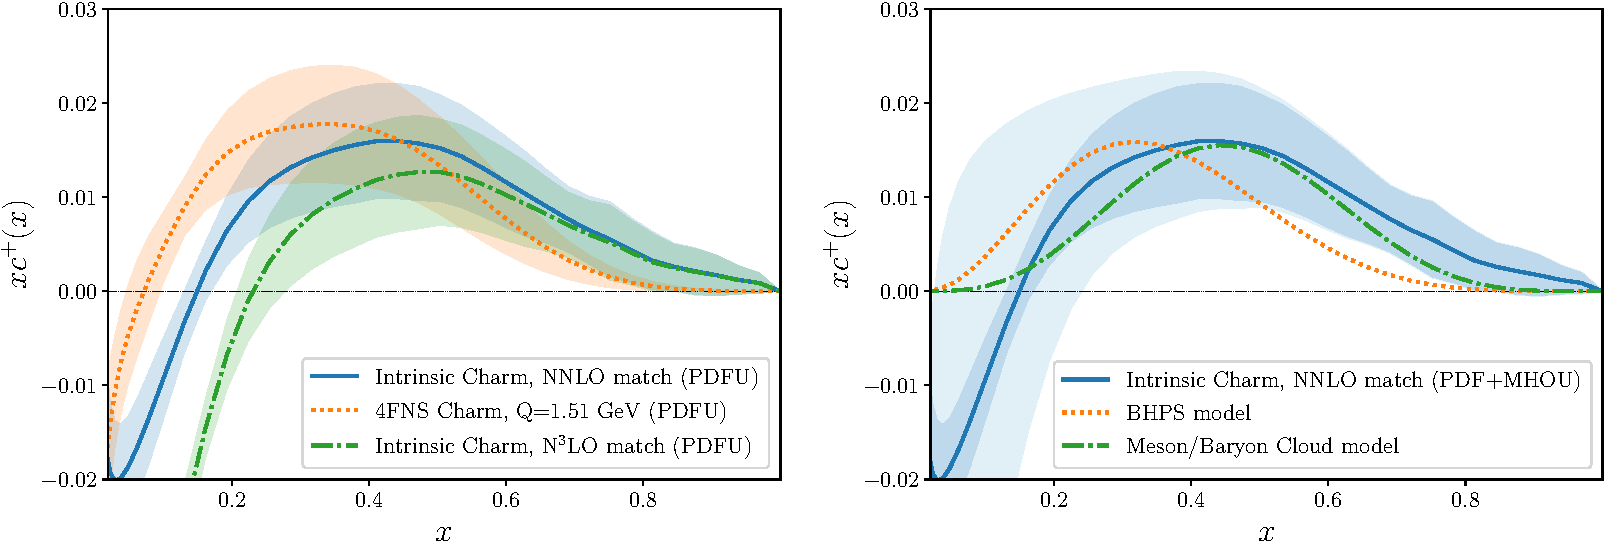
\includegraphics[width=0.99\linewidth]{ch-ic/Fig1.pdf}
    \caption{\small  \textbf{ The intrinsic charm \pdf
      and comparison with models}.
%
      Left: the purely
      intrinsic (3\fns) result (blue)
      with \pdf uncertainties only, compared to the 4\fns \pdf, that
      includes both an intrinsic and radiative
      component,   at
      $Q=m_c=1.51$ GeV (orange). The purely intrinsic (3\fns)
      result obtained using \nnnlo matching is also shown (green).
      %
      Right: the purely
      intrinsic (3\fns)
      final result with total uncertainty (\pdf+MHOU), with the \pdf
      uncertainty indicated as a dark shaded band;
the predictions from the original 
BHPS model~\cite{Brodsky:1980pb} and from the more recent meson/baryon
      cloud model~\cite{Hobbs:2013bia} are also shown for comparison
      (dotted and dot-dashed curves respectively).
         \label{fig:ic/charm_content_3fns} }
\end{center}
\end{figure}
%%%%%%%%%%%%%%%%%%%%%%%%%%%%%%%%%%%%%%%%%%%%%%%%%%%%%%%%%%%%%%%%%%%%%%

The intrinsic (3\fns) charm \pdf
displays a characteristic valence-like
 structure at large-$x$ peaking at $x\simeq 0.4$.
%
 While intrinsic charm is found to be small in absolute terms
 (it contributes less than 1\% to the proton  total momentum),
 it is significantly different from zero.
%
 Note that the transformation to the 3\fns has little effect on the peak region,
 because there is almost no charm radiatively generated at such large values of $x$: in
 fact, a very similar valence-like peak is already found in the 4\fns calculation.

Because at the charm mass scale the strong coupling $\alpha_s$ is rather
large, the perturbative expansion converges slowly.
%
In order to
estimate the effect of missing higher order uncertainties (MHOU), we
have also performed the transformation from the 4\fns \nnlo charm \pdf
determined from the data to the 3\fns (intrinsic) charm \pdf at one
order higher, namely at \nnnlo. 
%
The result is also shown
Fig.~\ref{fig:ic/charm_content_3fns} (left). Reassuringly, the intrinsic
valence-like structure is unchanged.
%
On the other hand, it is clear that for
$x\lsim 0.2$ perturbative uncertainties become very large.
%
We can estimate  the total uncertainty on our determination
of intrinsic charm by adding in quadrature the \pdf uncertainty and a
MHOU estimated from the shift between the result found using \nnlo
and \nnnlo matching.

This procedure leads to our final result for intrinsic charm and its total
uncertainty, shown in Fig.~\ref{fig:ic/charm_content_3fns} (right).
%
The intrinsic charm \pdf is found to be compatible with zero for
$x\lsim 0.2$: the negative trend 
seen  in Fig.~\ref{fig:ic/charm_content_3fns} with \pdf uncertainties only 
becomes 
compatible with zero upon inclusion of  theoretical
uncertainties. However, at
larger $x$ even with theoretical uncertainties
the intrinsic charm \pdf
 differs 
from zero by about 2.5 standard deviations ($2.5\sigma$) in the peak region.
%
This result  is stable upon variations of dataset, methodology (in
particular the \pdf  parametrization basis) and Standard Model
parameters (specifically the charm mass),
as demonstrated in the Supplementary Information (SI) Sects.~\ref{sec:ic/charm_stability_4fns}
and~\ref{sec:ic/charm_stability_3fns}. 

Our determination of intrinsic charm can be compared to theoretical expectations.
%
Subsequent to the
original intrinsic charm model of~\cite{Brodsky:1980pb} (BHPS
model),
a variety of other models were  
proposed~\cite{Hoffmann:1983ah,Pumplin:2005yf,Paiva:1996dd,Steffens:1999hx,Hobbs:2013bia},
see~\cite{Brodsky:2015fna} for a review.
%
Irrespective of their specific details, most models predict a valence-like
structure at large $x$ 
with a maximum located  between $x\simeq 0.2$ and $x\simeq 0.5$, and a
vanishing intrinsic component for
$x\lsim 0.1$.
%
In Fig.~\ref{fig:ic/charm_content_3fns}~(right) we compare our result to
the original BHPS model and to the more recent meson/baryon cloud model of~\cite{Hobbs:2013bia}.

As these models predict only the shape of the
intrinsic charm distribution, but not 
its overall normalization, we have normalized them by requiring
that they reproduce the same 
charm momentum fraction as our determination.
%
We find remarkable agreement between the shape of our 
determination and the model predictions.
%
In particular, we reproduce  the presence and location of the large-$x$ valence-like peak
structure (with  better agreement, of marginal statistical significance, with
the meson/baryon cloud calculation),  and the vanishing of 
intrinsic charm at small-$x$.
%
The fraction of the proton momentum carried by charm quarks that we
obtain from our analysis, 
used in this comparison to models,  is $\left( 0.62 \pm 0.28\right) \%$
including \pdf uncertainties only (see
SI Sect.~\ref{sec:ic/charm_mom_frac} for details).
%
However, the uncertainty
upon inclusion of MHOU greatly increases, and we obtain
$\left( 0.62 \pm 0.61\right) \%$, due to the contribution from the small-$x$
region, $x\lsim 0.2$, where the MHOU is very large, see
Fig.~\ref{fig:ic/charm_content_3fns}~(right).
%
%
Note that in most previous
analyses~\cite{Hou:2017khm} (see SI Sect.~\ref{sec:ic/ct}) intrinsic charm models (such as the BHPS
model) are fitted to the data, with only the momentum fraction left as
a free parameter.

We emphasize that in our analysis the charm \pdf is entirely
determined by the experimental data included in the \pdf determination.
The data with the most impact on charm are from recently measured \lhc
processes, which are both accurate and precise.
%
Since these measurements are made at high scales, the corresponding
hard cross-sections can be reliably computed in QCD perturbation theory.

Independent evidence for intrinsic charm
is provided by the very recent \lhcb measurements of $Z$-boson production
in association with charm-tagged jets in the forward
region~\cite{LHCb:2021stx}, which were not included in our baseline dataset.
%
This process, and specifically the ratio $\mathcal{R}_j^c$
of charm-tagged jets normalized to flavor-inclusive jets,
is directly sensitive to the charm \pdf~\cite{Boettcher:2015sqn}, and
with \lhcb kinematics also
in the kinematic region  where the  intrinsic component is relevant.
%
Following \cite{Boettcher:2015sqn,LHCb:2021stx}, we have  evaluated
$\mathcal{R}_j^c$ at \nlo~\cite{Alioli:2010xd,Sjostrand:2007gs} (cf.\
\cref{sec:ic/zcharm} for details), both with our default \pdfs that include
intrinsic charm, and also with an independent \pdf determination in which
intrinsic charm is constrained to vanish  identically, so charm is determined
by perturbative matching (cf.\ \cref{sec:ic/consistency}).

%%%%%%%%%%%%%%%%%%%%%%%%%%%%%%%%%%%%%%%%%%%%%%%%%%%%%%%%%%%%%%%%%%%
\begin{figure}[htbp]
  \begin{center}
    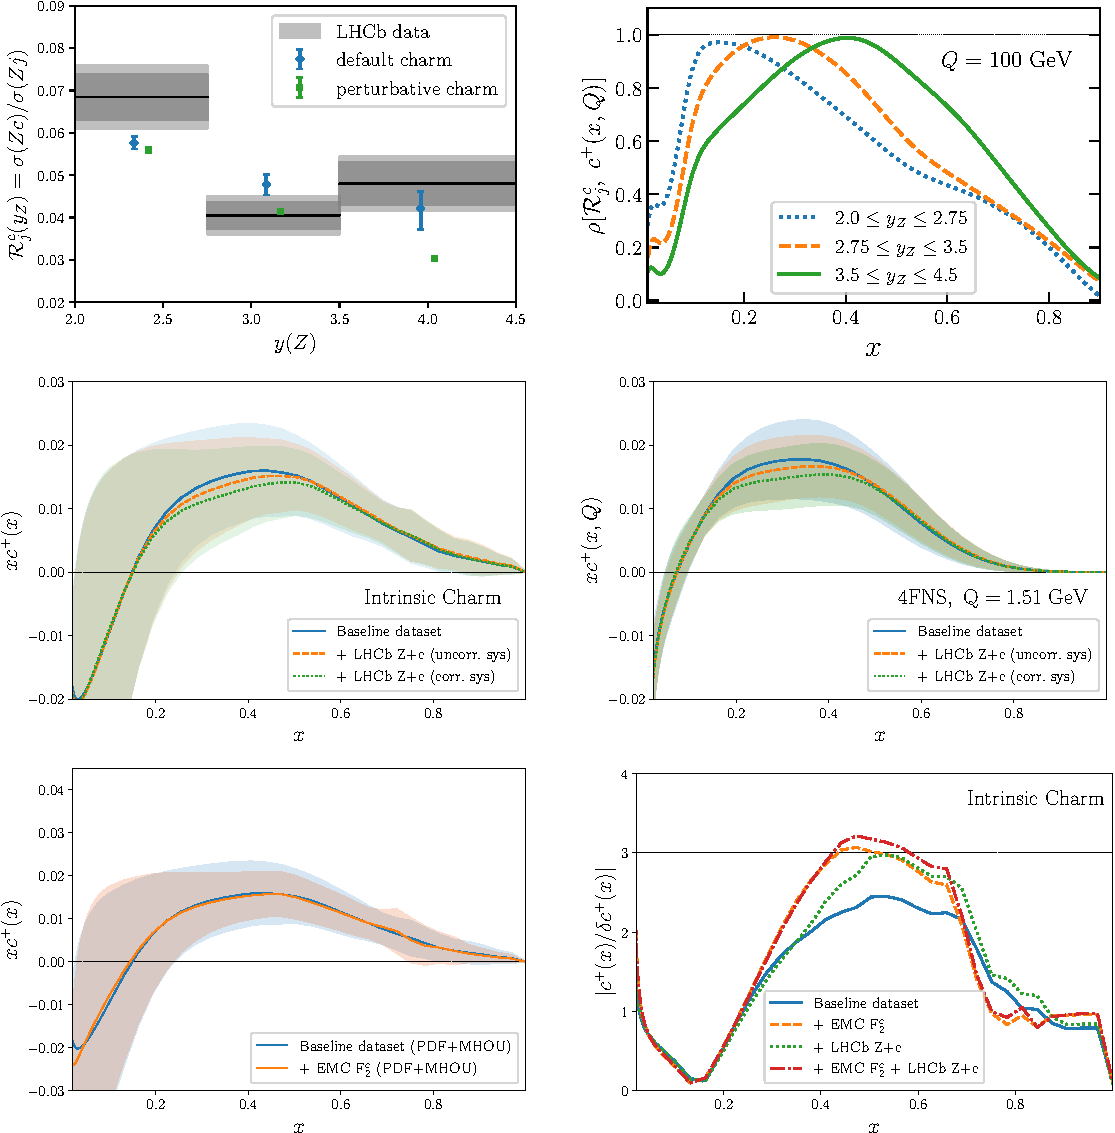
\includegraphics[width=0.99\linewidth]{ch-ic/Fig2.pdf}
     \caption{\small
       \textbf{ Intrinsic charm and $Z+$charm production at \lhcb.}
       %
       Top left: the \lhcb measurements of $Z$ boson production
      in association with charm-tagged jets, $\mathcal{R}_j^c$, at $\sqrt{s}=13$ TeV,  compared with
      our default prediction which includes an intrinsic charm component,
      as well as with a variant in which we impose the
      vanishing of the intrinsic charm component.
      %
       The thicker (thinner) bands in the \lhcb data indicate the statistical
      (total) uncertainty, while the theory predictions include both \pdf and MHO uncertainties.
      %
      Top right: the correlation coefficient between
     the  charm \pdf at $Q=100$ GeV in NNPDF4.0
      and the \lhcb measurements of $\mathcal{R}_j^c$ 
     for the three $y_Z$ bins.
      %
     Center: the charm \pdf
     in the 4\fns (right) and the intrinsic (3\fns) charm \pdf (left)
     before and after inclusion of the \lhcb $Z$+charm data.
     %
     Results are shown
     for both experimental correlation models discussed in the text.
     %
     Bottom left: the intrinsic charm \pdf before and after inclusion
     of the \emc charm structure function data.
     %
     Bottom right: the statistical significance of the
     intrinsic charm \pdf in our baseline analysis, compared to the results
     obtained also including either the \lhcb $Z$+charm (with uncorrelated
     systematics) or the \emc
     structure function data, or both.
  \label{fig:ic/Zc} }
\end{center}
\end{figure}
%%%%%%%%%%%%%%%%%%%%%%%%%%%%%%%%%%%%%%%%%%%%%%%%%%%%%%%%%%%%%%%%%%%%%%

In Fig.~\ref{fig:ic/Zc}~(top left) we compare the \lhcb measurements of $\mathcal{R}_j^c$, provided
in three bins of the $Z$-boson rapidity
$y_Z$, with the theoretical predictions
 based on both our default \pdfs as well as the \pdf set in
 which we impose the vanishing of intrinsic charm.
 %
 In Fig.~\ref{fig:ic/Zc}~(top right)
we also display the  correlation coefficient between
 the  charm \pdf at $Q=100$ GeV 
 and the observable  $\mathcal{R}_j^c$, demonstrating how this observable
 is highly
 correlated to charm in a localized
 $x$ region that depends on the rapidity bin.
 %
 It is clear that
 our prediction is in excellent agreement with the \lhcb measurements, while in the
 highest rapidity bin, which is highly correlated to the charm \pdf in
 the region of the observed valence peak $x\simeq 0.45$, the prediction
 obtained by imposing the vanishing of intrinsic charm undershoots the
 data at the $3\sigma$ level.
%
 Hence this measurement provides
 independent direct evidence in support of our result.

 We have also determined the impact of these \lhcb $Z$+charm measurements on the
charm \pdf.
%
Since the experimental covariance matrix is not available,
we have considered two limiting scenarios in which the total
systematic uncertainty is either completely uncorrelated 
($\rho_\textrm{ sys}=0$) or fully correlated  ($\rho_\textrm{ sys}=1$) between
 rapidity bins. The charm \pdf in the 4\fns before and after
inclusion of the \lhcb data (with either correlation model), and the intrinsic
charm \pdf obtained from it, are displayed in
Fig.~\ref{fig:ic/Zc}~(center left and right respectively).
%
The bands account for both \pdf and MHO uncertainties.
%
The results show full consistency: inclusion of the \lhcb  $\mathcal{R}_j^c$ data leaves
the intrinsic charm \pdf unchanged, while moderately reducing the
uncertainty on it.

In the past, the main indication for  intrinsic charm came from \emc data~\cite{Aubert:1982tt} on deep inelastic scattering with charm in the final state~\cite{Harris:1995jx}.
%
These data are relatively imprecise, their accuracy has often been questioned,
and they were taken at relatively low scales where radiative corrections are large.
%
For these reasons, we have not included them in our baseline
analysis.
%
However, it is interesting to assess the impact of
their inclusion.
%
Results are shown in 
Fig.~\ref{fig:ic/Zc}~(bottom left), where we display the
intrinsic charm \pdf before and after inclusion of the \emc data.
%
Just
like in the case of the \lhcb data we find full consistency: unchanged
shape and a moderate reduction of uncertainties.

We can summarize our results  through their so-called local statistical
significance, namely, the size of the intrinsic charm \pdf
in units of its total uncertainty.
%
This displayed  in Fig.~\ref{fig:ic/Zc}~(bottom right) for our default determination of
intrinsic charm, as well as after inclusion of either the \lhcb $Z$+charm or the
\emc data, or both.
%
We find a local significance for intrinsic charm at the $2.5\sigma$ level
in the region $0.3 \lsim x \lsim 0.6$.
%
This is increased to about
$3\sigma$ by the inclusion of either the \emc or the \lhcb
data, and above if they are both included.
%
The similarity of the impact of the \emc and \lhcb measurements is
especially remarkable in view of the fact that they involve very
different physical processes and energies.
